\secnumbersection{Propuesta de solución}

\subsection{Comprensión del problema}

Inicialmente sabemos que los elementos inválidos podrían encontrarse luego de refinar una malla Octree con diferentes niveles de refinamiento, específicamente en el límite donde se producen las transiciones entre regiones de diferente nivel de refinamiento.

Estos elementos inválidos podremos identificarlos por su $J_{ENS}$ menor a cero. Entonces se ejecutó \textit{JENS\_GENERATOR} a la malla inicial y se obtuvo la estadística de calidad de los elementos de la malla inicial, \autoref{out:jens_output_c_5r7_0}.

Nos enfocaremos sólo en elementos inválidos, por lo tanto, el threshold a estudiar será cero.

Para ello se realizó una pequeña modificación a \textit{MESHER\_GENERATOR} y al final de su algoritmo, cuando se exportan los datos de la malla, en específico, cuando guardan los puntos, elementos y octantes de la malla, se realiza una identificación de los índices de elementos que pertenecen a cada octante y se guardan en su clase como información del octante.

Para guardarlo en el octante se agrega un atributo a la clase llamado \textit{sub\_elements\_indexes}, línea 16 en \autoref{code:octant_class_modification}.

Este atributo es consultado después, cuando se etiqueta cada octante que presente elementos inválidos.

\begin{lstlisting}[style=CStyle,caption={Modificación Clase Octant.\\ Fuente: Elaboración propia.},label={code:octant_class_modification}]
#include <vector>
class Octant
{
	public:
        Octant(vector<unsigned int> &epts, const unsigned short &ref_level,
    			   const unsigned int &o_id);
        ...
        // indice del octante.
        unsigned int id;
        // indices de puntos que conforman al octante.
        vector<unsigned int> points_indexes;
        // indices de puntos que conforman los elementos 
        // pertencientes al octante.
        vector<vector<unsigned int>> sub_elements_points_indexes;
        // indices de elementos pertenecientes al octante.
        vector<unsigned int> sub_elements_indexes; 
}
\end{lstlisting}
Actualmente, hemos identificado 27 elementos que necesitan mejoras, pero aún no se ha determinado cuáles son específicamente esos elementos. Para resolver este problema, es necesario que el algoritmo \textit{MESHER\_GENERATOR} incluya una funcionalidad para etiquetar los elementos inválidos.

Se propone, de manera similar a \cite{daines2018repairing}, implementar un marcador para los octantes que contengan elementos de mala calidad, basado en una cota superior predefinida, como se muestra en \autoref{alg:get_labeled_octants}.

% Se propone, de manera similar a \cite{daines2018repairing}, un marcador de octantes que contienen elementos de mala calidad dada una cota superior, \autoref{alg:get_labeled_octants}.

Esta técnica permitirá identificar los octantes que necesitan ser refinados en etapas posteriores. En esta fase, nos enfocamos en identificar los elementos contenidos dentro de estos octantes.

Así, al obtener la lista de octantes involucrados, ahora es posible obtener los índices de los elementos que los componen, permitiendo su posterior análisis.


\begin{algorithm}
\caption{Algoritmo para etiquetar octantes que contienen elementos con peor calidad que la cota entregada.}\label{alg:get_labeled_octants} 
\SetKwInOut{KwIn}{Input}
\SetKwInOut{KwOut}{Output}
% functions
\SetKwFunction{getLabeledOctants}{GET\_LABELED\_OCTANTS}
\SetKwFunction{calculateJens}{CALCULATE\_JENS}
\SetKwFunction{getOctant}{GET\_OCTANT}
\SetKwFunction{getIndex}{GET\_INDEX}
\SetKwFunction{add}{ADD}
% procedure
\SetKwProg{myproc}{Procedure}{:}{}
\KwIn{Refinement level constraints $RLC$, triangular surface mesh \Omega, quality threshold $T$, maximum number of iterations $I$.}
\KwOut{if successful, volumetric mesh of \Omega that meet the $RLC$ with quality greather than $T$.}
\myproc{\getLabeledOctants{$M$, $T$}}
{
    $lo$ \gets \, $empty set$ \;
    \For{ \textbf{each} $element$ \textbf{in} $M$} {
        $q$ \gets \, \calculateJens{$element$}\;
        \If{$q < T$} {
            $octant$ \gets \, $element$.\getOctant{}\;
            $octant\_index$ \gets \, $octant$.\getIndex{}\;
            $lo$.\add{$octant\_index$}\;
        }
    }
    \KwRet $lo$\;    
}
\end{algorithm}

Utilizando la lista de elementos involucrados, podemos visualizar los resultados en ParaView. Esto nos permite generar la \autoref{fig:cortex_surf_oct_labeled}, donde los elementos pertenecientes a los octantes afectados se destacan en color verde. 

Con esta visualización, podemos confirmar que estos elementos se encuentran en la vecindad de las transiciones entre regiones con distintos valores de $RL$. Esta representación clara facilita la identificación de las áreas problemáticas dentro de la malla y demuestra cómo las transiciones entre regiones con diferentes características influyen en la calidad de los elementos.

% \begin{algorithm}
% \caption{Modificación del algoritmo para etiquetar octantes, permite imprimir en consola los elementos que forman cada octante etiquetado.}\label{alg:get_labeled_octants_modification} 
% \SetKwInOut{KwIn}{Input}
% \SetKwInOut{KwOut}{Output}
% % functions
% \SetKwFunction{getLabeledOctants}{GET\_LABELED\_OCTANTS}
% \SetKwFunction{calculateJens}{CALCULATE\_JENS}
% \SetKwFunction{getOctant}{GET\_OCTANT}
% \SetKwFunction{getIndex}{GET\_INDEX}
% \SetKwFunction{getSubElementIndexes}{GET\_SUB\_ELEMENTS\_INDEXES}
% \SetKwFunction{add}{ADD}
% \SetKwFunction{size}{SIZE}
% % procedure
% \SetKwProg{myproc}{Procedure}{:}{}
% \KwIn{Malla Octree $M$, cota de calidad $T$.}
% \KwOut{Lista de Octantes con elementos de mala calidad etiquetados.}
% \myproc{\getLabeledOctants{$M$, $T$}}
% {
%     $lo$ \gets \, empty set \tcp*{Lista de Octantes etiquetados.} 
%     \For{ \textbf{each} $element$ \textbf{in} $M$} {
%         $q$ \gets \, \calculateJens{$element$}\;
%         \If{$q < T$} {
%             $octant$ \gets \, $element$.\getOctant{}\;
%             $octant\_index$ \gets \, $octant$.\getIndex{}\;
%             $lo$.\add{$octant\_index$}\;
%             $le$ \gets \, $octant$.\getSubElementIndexes{}\;
%             \textbf{PRINT} octant: $octant\_index$ \;
%             \textbf{subelements:} \;
%             \For{ $k \gets 0$ to $le$.\size{} } {
%                 \textbf{PRINT} $le_{k}$
%             }
%         }
%     }
%     \KwRet $lo$\;    
% }
% \end{algorithm}

\begin{figure}[!ht]
    \centering
    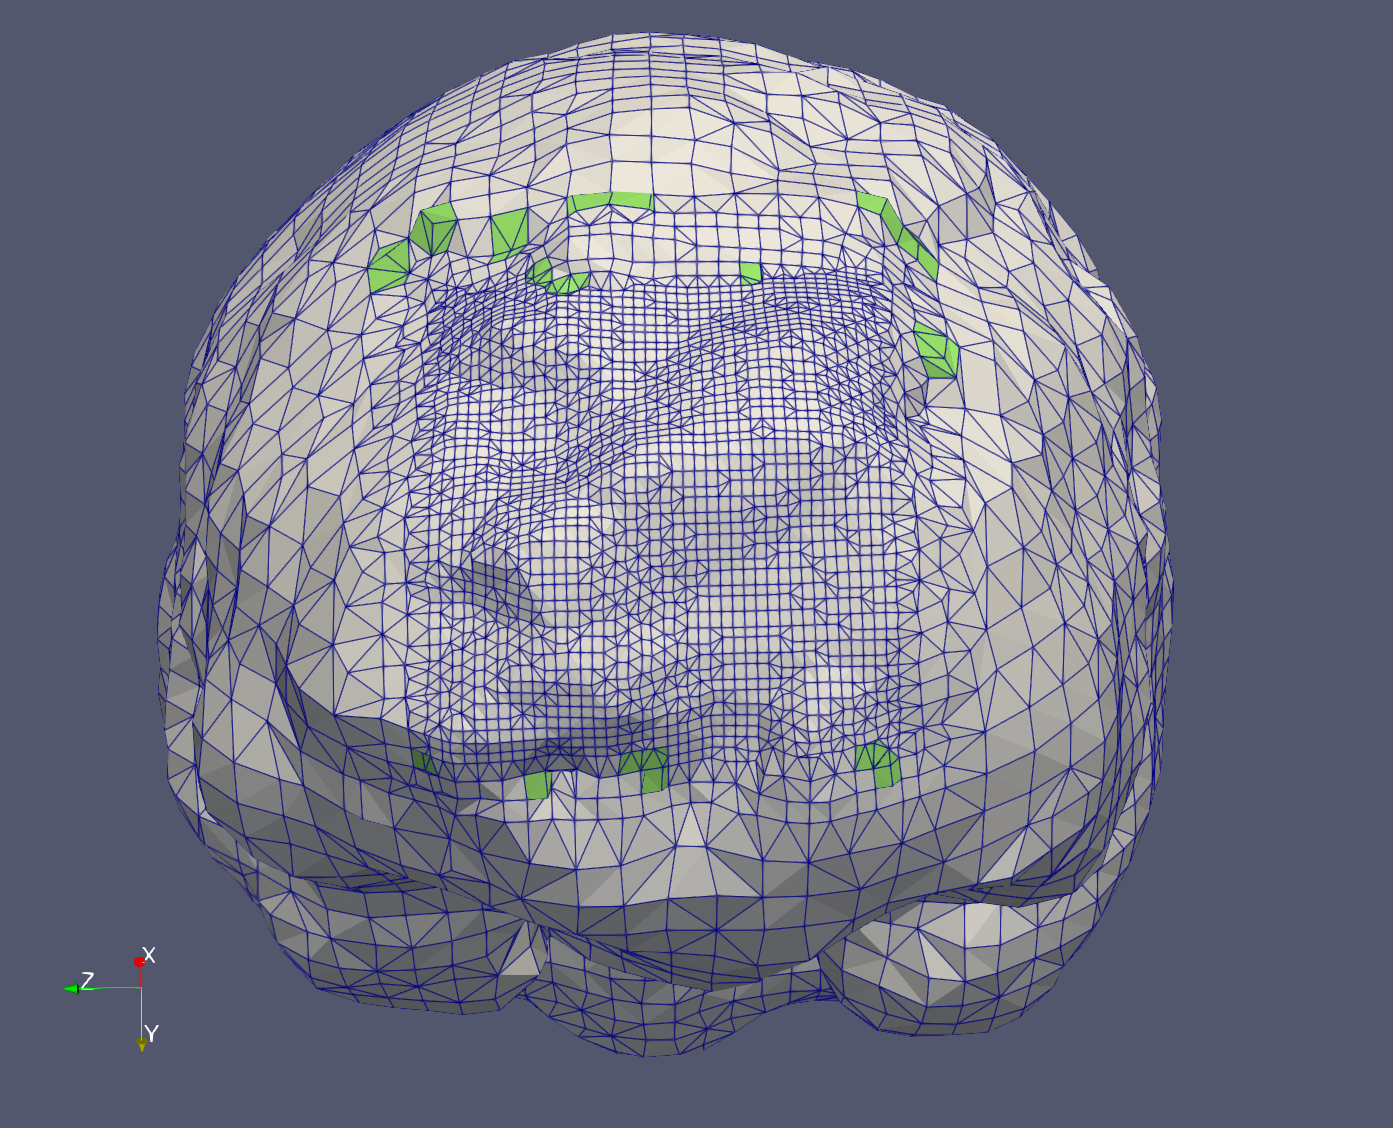
\includegraphics[width=0.6\textwidth]{figures/labeled_octs/labeled_oct_c_5r7_0.png}
    \caption{ Zona frontal de la malla donde se presentan los elementos inválidos (verde). }
    Fuente: Elaboración propia.
    \label{fig:cortex_surf_oct_labeled}
\end{figure}

\subsection{Comprensión de elementos inválidos}

Para comprender mejor el problema, se realizará un análisis gráfico localizado, centrándose en un octante específico situado en la parte inferior izquierda del frontis de la malla. Este octante ha sido seleccionado debido a su característica cóncava en la superficie y porque contiene varios elementos inválidos. Además, se encuentra en la intersección de dos regiones que requieren refinamiento, cada una con diferentes valores de $RL$.

En la \autoref{fig:zoom_cortex_surf}, se presenta la región de interés en el contexto de la malla inicial. La imagen a la izquierda muestra la malla en su totalidad, mientras que la imagen a la derecha proporciona una vista ampliada de la zona aislada del octante afectado. En esta vista detallada, se pueden observar todos los elementos contenidos en dicho octante, con los elementos inválidos resaltados en verde. 


\begin{figure}[!ht]
    \centering
    \begin{subfigure}[t]{0.45\textwidth}
        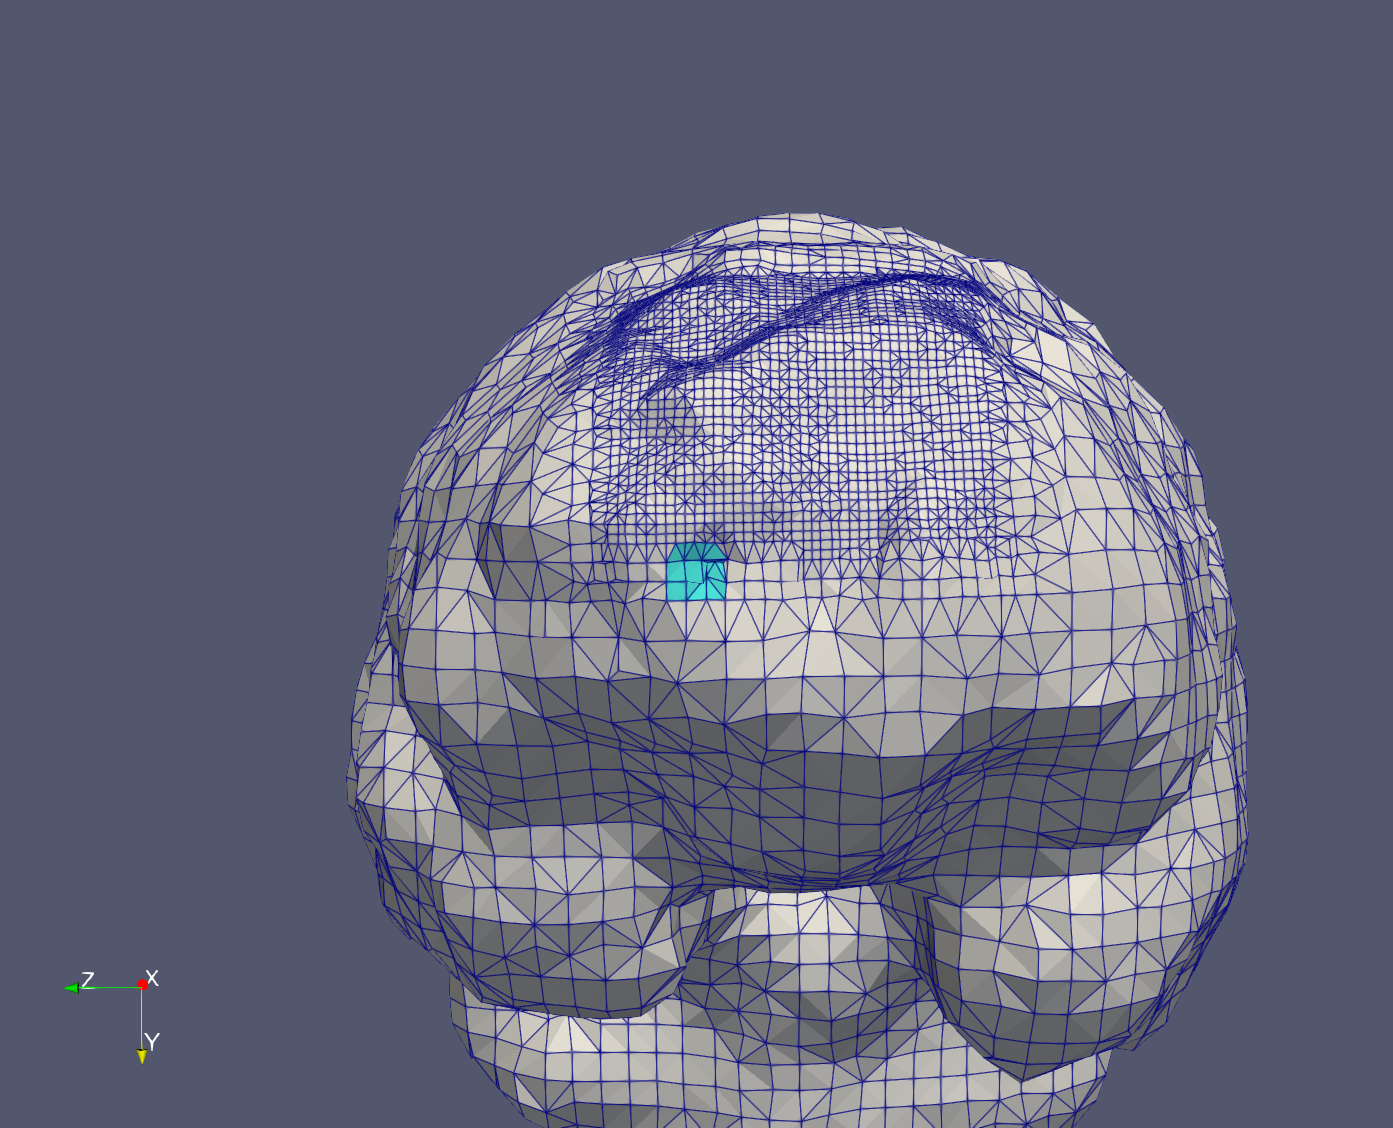
\includegraphics[width=1.0\textwidth]{figures/bad_quality_zone/zoom_out_bq_zone.png}
        \caption{Zoom out de sección extraída.}
    \end{subfigure}
    \begin{subfigure}[t]{0.45\textwidth}
        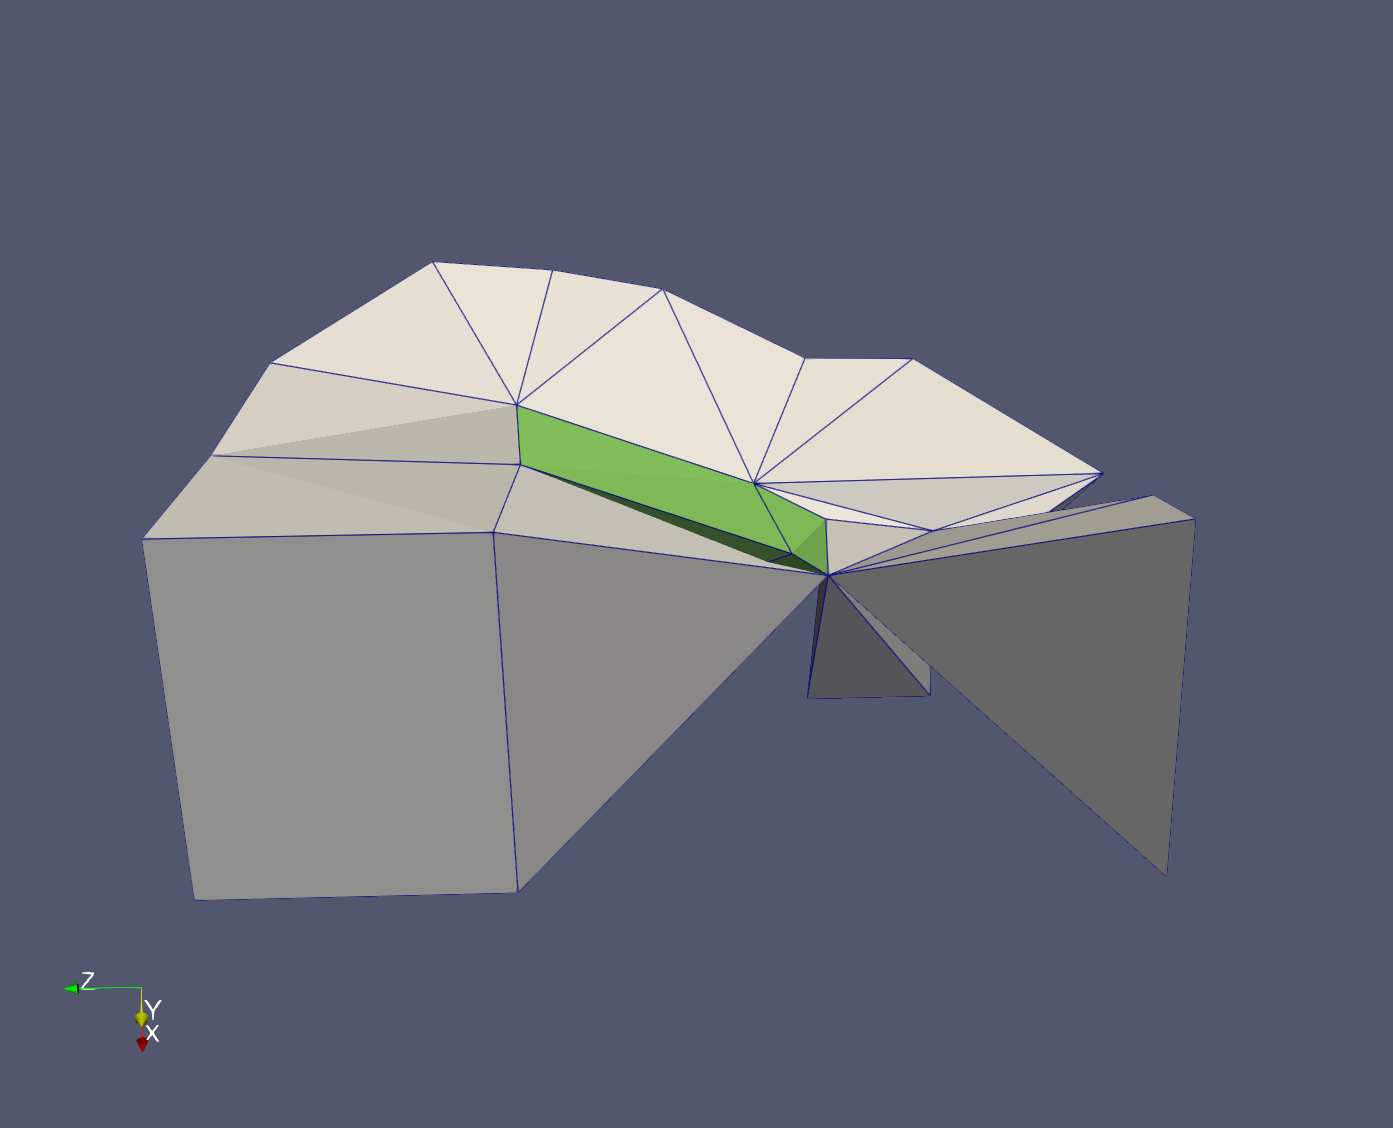
\includegraphics[width=1.0\textwidth]{figures/bad_quality_zone/bq_zone_02.png}
        \caption{Zona extraída con elementos de mala calidad resaltados.}
    \end{subfigure}
    \caption{ Zona a analizar para evidenciar elementos de mala calidad, esta zona se extrajo de la representación de la malla con un nivel 5 de refinamiento general y nivel 7 de refinamiento en la superficie entregada. En la imagen de la izquierda se muestra una visión general de la superficie de la malla demarcada por elementos con vértices azules y la zona a estudiar de color celeste. En la imagen de la derecha, la zona a estudiar y un par de elementos de mala calidad destacados con color verde. }
    Fuente: Elaboración propia.
    \label{fig:zoom_cortex_surf}
\end{figure}

% \begin{algorithm}
% \caption{Algoritmo para etiquetar elementos.}\label{alg:get_labeled_elements} 
% \SetKwInOut{KwIn}{Input}
% \SetKwInOut{KwOut}{Output}
% % functions
% \SetKwFunction{getLabeledElements}{GET\_LABELED\_ELEMENTS}
% \SetKwFunction{calculateJens}{CALCULATE\_JENS}
% \SetKwFunction{getOctant}{GET\_OCTANT}
% \SetKwFunction{getIndex}{GET\_INDEX}
% \SetKwFunction{getSubElementIndexes}{GET\_SUB\_ELEMENTS\_INDEXES}
% \SetKwFunction{add}{ADD}
% \SetKwFunction{size}{SIZE}
% % procedure
% \SetKwProg{myproc}{Procedure}{:}{}
% \KwIn{Malla Octree $M$, cota de calidad $T$.}
% \KwOut{Lista de Elementos de mala calidad etiquetados.}
% \myproc{\getLabeledElements{$M$, $T$}}
% {
%     $le$ \gets \, empty set \tcp*{Lista de Elementos etiquetados.} 
%     \For{ \textbf{each} $element$ \textbf{in} $M$} {
%         $q$ \gets \, \calculateJens{$element$}\;
%         \If{$q < T$} {
%             $element\_index$ \gets $element$.\getIndex{}\;
%             $le$.\add{$element\_index$}\;
%         }
%     }
%     \KwRet $lo$\;    
% }
% \end{algorithm}

\subsection{Análisis de la vecindad}

En esta sección de la malla, se puede observar a simple vista una superficie de naturaleza cóncava. Este tipo de geometría tiende a facilitar la aparición de elementos inválidos durante el proceso de generación de la malla.

Como se muestra en la \autoref{fig:zoom_cortex_surf_all}, los elementos inválidos son fácilmente identificables. Estos elementos, destacados en verde, crean áreas en la malla que no representan fielmente la geometría original y muestran incongruencias respecto a los elementos vecinos. En este contexto, los elementos inválidos generan una anomalía observable en relación a su entorno inmediato.

En particular, el par de elementos en verde está separado de los elementos adyacentes en su base. Esta separación indica una ruptura en la continuidad de la malla que no sigue la forma esperada de la superficie original. Este análisis resalta la importancia de prestar atención a la forma y las transiciones entre regiones de la malla para detectar y corregir estos problemas que pueden comprometer la calidad y precisión de la representación del modelo.

\begin{figure}[!ht]
    \centering
    \includegraphics[width=1.0\textwidth]{figures/bad_quality_zone/bq_zone_ALL.png}
    \caption{ Perspectivas de vecindario (gris) donde se encuentra un para de elementos inválidos (verde). }
    Fuente: Elaboración propia.
    \label{fig:zoom_cortex_surf_all}
\end{figure}


\subsection{Propuesta}

Para abordar y mejorar la calidad de los elementos inválidos en la malla, se propone refinar las localidades donde estos se encuentran. En términos específicos, esto implica realizar un refinamiento en los octantes que están asociados con los elementos inválidos.

% Entonces, en general, se necesitará luego de generar la malla, identificar y etiquetar los octantes que contengan elementos inválidos.  

% Luego, iterar nuevamente la malla para refinar aquellos octantes identificados y realizar las transformaciones pertinentes para mantener la congruencia en la malla.

% Realizar las iteraciones de los pasos anteriores las veces necesarias hasta obtener una malla congruente, sin elementos inválidos.

Se definirá el algoritmo de esta propuesta como el siguiente:

\begin{enumerate}
    \item Generación de malla inicial.
    
        La generación de la malla inicial implica utilizar el \textit{MESHER\_GENERATOR} para construir la malla, con $RL_{gral} = 5$ y $R_{surf} = 7$. 
    \item Identificación y Etiquetado de Octantes.
        
        El \autoref{alg:get_labeled_octants} que incluye la funcionalidad \textit{GET\_LABELED\_OCTANTS}, facilitará cumplir con esta etapa del algoritmo.
    \item Refinamiento de Octantes Identificados.
        
        El refinamiento de una lista de octantes puede realizarse con una de las funcionalidades de \textit{MESHER\_GENERATOR}.
    \item Ciclo Iterativo de Evaluación y Refinamiento.
        
        Para realizar el proceso de iteración, se construirá un script en bash que ejecute \textit{MESHER\_GENERATOR} con ciertas condiciones.
\end{enumerate}

\subsubsection{Generación de malla inicial.}


\begin{lstlisting}[style=Console,caption={Generador de malla, crea una malla refinada a nivel 5 y especificamente refina la superficie entregada a nivel 7, se exportará la malla con el nombre \textit{c\_5r7\_0}, en formato vtk y m3d.\\ Fuente: Elaboración propia.}]
input  >    ./mesher_roi -d ./data/cortex.mdl -s 5 -r ./data/cortex_surf_roi.mdl 7 -u c_5r7_0 -m -v
output >    All done in xxxx ms
\end{lstlisting}

% Para preparar esta malla inicial para su mejora, se realizó una modificación al algoritmo de \textit{MESHER\_GENERATOR}, permitiendo obtener, al finalizar la generación de la malla, estadísticas $J_{ENS}$ con la frecuencia de elementos, segunda columna en \autoref{code:jens_histo_c_5r7_0}, con $J_{ENS}$ menor a las cotas dispuestas en la primera columna.

% Esto se implementó exportando la información en un archivo con extensión '.histo', el histograma generado en \textit{JENS\_STADISTICS\_GENERATOR} y de esta manera, también lograr gestionar la información de forma óptima entre sistemas de información.

% Además, por defecto, \textit{MESHER\_GENERATOR} crea un archivo de respaldo con extensión '.oct' que guarda información de la malla, sus puntos y octantes definidos en la iteración.
Para mejorar la calidad de la malla inicial, se implementaron modificaciones específicas en el algoritmo \textit{ MESHER\_GENERATOR}. Estas modificaciones están diseñadas para evaluar y gestionar la calidad de los elementos generados, proporcionando estadísticas detalladas y facilitando la integración con otros sistemas de información.
Se ha actualizado el algoritmo \textit{MESHER\_GENERATOR} para que, al finalizar la generación de la malla, se obtengan estadísticas de calidad $J_{ENS}$. Estas estadísticas se presentan en un formato que permite evaluar la calidad de los elementos en relación con ciertos umbrales predeterminados, además se modificó la información sobre los octantes que se guardan de manera persistente en el disco en \textit{MESHER\_GENERATOR}.

Puntos a destacar de esta implementación:
    
\begin{itemize}
    \item  Generación de Estadísticas $J_{ENS}$:

    Al finalizar la generación de la malla, el algoritmo calcula las estadísticas $J_{ENS}$. Estas estadísticas proporcionan una medida de la calidad de los elementos de la malla y se registran en cada iteración, creando un historial detallado de calidad. Este proceso es crucial para monitorizar y evaluar la calidad de la malla generada de forma continua.

    \item Exportación de datos en formato estándar:
    
    % Para facilitar el análisis de las estadísticas $J_{ENS}$, se guardarán en un archivo con extensión \textbf{.histo} de manera persistente donde la primera columna representará las cotas de calidad y la segunda columna mostrará la frecuencia de elementos cuya calidad es inferior a las cotas de la primera columna. Esto se ilustra en la \autoref{code:jens_histo_c_5r7_0}.

    % En este archivo de muestra, se dispondrán las cotas en la primera fila, se comenzará por la cota de elementos con $J_{ENS}$ negativo, luego se seguirá con una cota $0.03$ y $0.05$ para posteriormente incrementar a intervalos regulares de dimensión $0.05$.
    
    % Esto corresponde al histograma generado por el módulo \textit{JENS\_STATISTICS\_GENERATOR}, el cual permite visualizar y analizar de manera eficiente la distribución de la calidad de los elementos dentro de la malla.

Para facilitar el análisis de las estadísticas $J_{ENS}$, los datos se almacenarán de manera persistente en un archivo con la extensión .histo. Este archivo estructurado contiene dos columnas esenciales para la evaluación de la calidad de la malla. En la primera columna, se registrarán los umbrales o cotas de calidad, mientras que la segunda columna mostrará la frecuencia de elementos cuya calidad está por debajo de cada umbral específico. La estructura de este archivo se ilustra en la \autoref{code:jens_histo_c_5r7_0}.

En el archivo \textbf{.histo}, las cotas se dispondrán en la primera fila comenzando por una cota que incluye los elementos con $J_{ENS}$ negativo. A continuación, se utilizarán cotas progresivas como $0.03$ y $0.05$, seguidas de incrementos regulares de $0.05$. Este formato de incremento permite una evaluación granular y sistemática de la calidad de los elementos a lo largo de un rango definido de valores $J_{ENS}$.

El histograma contenido en el archivo es generado por el módulo \textit{JENS\_STATISTICS\_GENERATOR}. Este módulo es crucial porque facilita la visualización y el análisis eficiente de la distribución de la calidad de los elementos dentro de la malla. Al proporcionar una representación clara y estructurada de cómo se distribuye la calidad de los elementos, el histograma ayuda a identificar rápidamente cómo se ven afectados los elementos de la malla al realizar cada iteración.
    
\begin{lstlisting}[style=TxtStyle,caption={Estructura de archivo con extensión \textit{.histo} que contiene un histograma con estádisticas de elementos $J_{ENS}$ de la malla de la iteración actual.\\ Fuente: Elaboración propia.},label={code:jens_histo_c_5r7_0}]
____________________________________________
 File: c_5r7_x.histo 
____________________________________________
negative <neg_fq_bqe>
0.030000 <0.03_fq_bqe>
0.050000 <0.05_fq_bqe>
0.100000 <0.10_fq_bqe>
0.150000 <0.15_fq_bqe>
0.200000 <0.20_fq_bqe>
0.250000 <0.25_fq_bqe>
0.300000 <0.30_fq_bqe>
0.350000 <0.35_fq_bqe>
0.400000 <0.40_fq_bqe>
0.450000 <0.45_fq_bqe>
0.500000 <0.50_fq_bqe>
0.550000 <0.55_fq_bqe>
0.600000 <0.60_fq_bqe>
0.650000 <0.65_fq_bqe>
0.700000 <0.70_fq_bqe>
0.750000 <0.75_fq_bqe>
0.800000 <0.80_fq_bqe>
0.850000 <0.85_fq_bqe>
0.900000 <0.90_fq_bqe>
0.950000 <0.95_fq_bqe>
1.000000 <1.00_fq_bqe>
\end{lstlisting}

    \item Gestión de información entre sistemas:

    La exportación en formato \textbf{.histo} también permite una integración óptima de la información entre diferentes sistemas de procesamiento y análisis.
    Esta gestión eficiente asegura que los datos de calidad de la malla sean accesibles y utilizables en otras aplicaciones o modificaciones al algoritmo en trabajos futuros, facilitando así el flujo de trabajo en entornos complejos de simulación o modelado.
    
    \item Respaldo de la información de la malla:
    
    Además de las estadísticas de calidad, se necesitará disponer de un estado de la malla, por defecto, \textit{MESHER\_GENERATOR} crea un archivo de respaldo de extensión \textit{.oct}, que contiene una representación detallada de la malla, incluyendo la posición de los puntos y la definición de los octantes en cada iteración.
    Este archivo es esencial para conservar un registro completo del estado de la malla en diferentes etapas del proceso de generación de la malla y su refinamiento.

    Este archivo de respaldo, será modificado para incluir información adicional sobre los octantes, para posteriormente localizar correctamente octantes en base a sus identificadores únicos.
    
    Este archivo \textit{.oct} permite una fácil recuperación y revisión de la malla generada, facilitando la identificación de problemas y la evaluación de la calidad en etapas posteriores.
    También sirve como un recurso valioso para la documentación y el seguimiento de los cambios realizados durante el proceso de refinamiento de la malla.
\end{itemize}
    




% \begin{lstlisting}[style=TxtStyle,caption={Histograma con estádisticas de elementos Jens en malla inicial.\\ Fuente: Elaboración propia.},label={code:jens_histo_c_5r7_0}]
% ____________________________________________
%  File: c_5r7_0.oct 
% ____________________________________________
% <np> <ne> <no>

% <p_0_x> <p_0_y> <p_0_z>
% <p_1_x> <p_1_y> <p_1_z>
% <p_2_x> <p_2_y> <p_2_z>
% ...
% <p_NP-2_x> <p_NP-2_y> <p_NP-2_z>
% <p_NP-1_x> <p_NP-1_y> <p_NP-1_z>
% <p_NP_x> <p_NP_y> <p_NP_z>

% <octedpid_0_x> <octedpid_0_y> <ed_0_id>
% <octedpid_1_x> <octedpid_1_y> <ed_1_id>
% ...
% <octedpid_ED-1_x> <octedpid_ED-1_y> <ed_ED-1_id>
% <octedpid_ED_x> <octedpid_ED_y> <ed_ED_id>

% <npo_0> <pid_0_0> ... <pid_0_NPO_0> <rl_0> <octid_0>
% <nif_0> <if_0_0> ... <if_0_NIF_0>
% <npo_1> <pid_1_0> ... <pid_1_NPO_0> <rl_1> <octid_1>
% <nif_1> <if_1_0> ... <if_1_NIF_1>
% ...
% <npo_NO-1> <pid_NO-1_0> ... <pid_NO_NPO_0> <rl_NO> <octid_NO-1>
% <nif_NO-1> <if_NO-1_0> ... <if_NO-1_NIF_NO-1>
% <npo_NO> <pid_NO_0> ... <pid_NO_NPO_0> <rl_NO> <octid_NO>
% <nif_NO> <if_NO_0> ... <if_NO_NIF_NO-1>

% Geometric Transform
% <centroid_x> <centroid_y> <centroid_z>
% <coord_x> <coord_y> <coord_z>

% <octmeshid_0> <octmeshid_1>...<octmeshid_NO-1> <octmeshid_NO>
% \end{lstlisting}

% \begin{lstlisting}[style=TxtStyle,caption={Histograma con estádisticas de elementos Jens en malla inicial.\\ Fuente: Elaboración propia.},label={code:jens_histo_c_5r7_0}]
% ____________________________________________
%  File: c_5r7_0.oct 
% ____________________________________________
% 143105 598817 122438

% +2.85692000E-01  +2.21920000E-02  +1.91885460E+01
% +1.34949800E+02  +2.21920000E-02  +1.91885460E+01
% ...
% +1.37053927E+02  +9.04996396E+01  +6.33752064E+01
% +1.37053927E+02  +9.04996396E+01  +1.09665994E+02

% 0 1 21
% 0 3 22
% ...
% 142878 142879 0
% 142880 142881 0

% 8 37427 37436 37441 37439 22347 37431 37440 37434 7 34256
% 3 4491 4615 4723
% 8 37436 37428 37437 37441 37431 22339 37432 37440 7 34257
% 2 4615 4723
% ...
% 8 142881 142871 142868 142880 22312 22231 1134 22311 4 147370
% 0
% 8 142876 142881 142880 142875 22304 22312 22311 5201 4 147371
% 0

% Geometric Transform
% 0.000000 0.000000 0.000000
% 0.000000 0.000000 0.000000

% 0 0 1 ... 1 1 1 
% \end{lstlisting}

\subsubsection{Identificación y etiquetado de Octantes.}

Como se explicó en la sección de \textit{Análisis de la vecindad}, identificar y etiquetar los octantes se realizará por medio del algoritmo \ref{alg:get_labeled_octants}, adicional a esto, se creará un archivo con la extensión \textit{.ref} para persistir la información. Este archivo es crucial porque almacenará una lista detallada de los índices de los octantes que necesitan ser refinados. Es importante que esta lista sea persistente para, además de tener un historial de los octantes refinados en cada iteración, lograr convalidarlo con el trabajo existente en \textit{MESHER\_GENERATOR}.

La persistencia de esta información permite rastrear los cambios realizados en cada iteración del refinamiento, asegurando una documentación completa y accesible del proceso. Facilita la revisión y análisis posterior pudiendo incluso, utilizar otros lenguajes de programación en el proceso.

\begin{lstlisting}[style=TxtStyle,caption={Lista de octantes a refinar en malla inicial.\\ Fuente: Elaboración propia.},label={code:oct_labeled_c_5r7_0}]
____________________________________________
 File: c_5r7_x.ref 
____________________________________________
<octid_0>
<octid_1>
...
<octid_NOL-1>
<octid_NOL>
\end{lstlisting}

En \autoref{code:oct_labeled_c_5r7_0}, se dispone un ejemplo del archivo \textit{.ref}, considerando $NOL$ la cantidad de octantes a refinar y $octid\_k$ los identificadores únicos de los octantes a refinar, siendo $k \in \{ 0, ..., NOL\}$.

\subsubsection{Refinamiento de Octantes Identificados.}

Teniendo en consideración la lista de octantes a refinar exportado en el archivo \textit{.ref}, queda entonces entregar esta lista a \textit{MESHER\_GENERATOR}, junto con el listado debe entregarse también la malla de la iteración anterior.

De esta manera, en una posible iteración 3, por ejemplo, se utilizará el archivo \textit{.oct} y \textit{.ref} de la iteración 2, esto es comenzar con la malla generada en la iteración anterior como en \autoref{code:ref_oct_labeled_iter_3}, donde se definen los siguientes elementos:

\begin{itemize}
    \item \textit{-d ./data/cortex.mdl}: Corteza del cerebro a analizar. 
    \item \textit{-c c\_5r7\_2.oct}: Información sobre los octantes generados en la iteración anterior.
    \item \textit{-l ./c\_5r7\_2.ref}: Lista de Octantes a refinar.
    \item \textit{-t 0.0}: Treshold definido en cero.
    \item \textit{-u c\_5r7\_3}: Nombre base de los archivos a exportar en la iteración actual.
    \item \textit{-m}: Exportación en formato m3d.
    \item \textit{-v}: Exportación en formato vtk.
\end{itemize}

Lo anterior, refinará los Octantes de mala calidad de la malla en la iteración 2 según la cota definida en dicha iteración y analizará los nuevos elementos para definir una nueva lista de Octantes a refinar.
Esto se exportará con el nombre de la iteración actual, exportando los siguientes archivos.

\begin{itemize}
    \item \textit{c\_5r7\_3.oct}: Información sobre los puntos y octantes de la malla generada,
    \item \textit{c\_5r7\_3.ref}: Lista de Octantes a refinar en iteración actual.
    \item \textit{c\_5r7\_3.m3d}: Información sobre puntos, elementos y octantes de la malla generada para visualización en Geomview.
    \item \textit{c\_5r7\_3.vtk}: Información sobre puntos, elementos y octantes de la malla generada para visualización en Paraview.
\end{itemize}


\begin{lstlisting}[style=Console,caption={Generador de malla, crea una nueva malla, tomando como input la malla inicial \textit{c\_5r7\_0.oct}, la lista de octantes a refinar \textit{c\_5r7\_0.ref}, la cota de calidad $J_{ENS}$ definido en cero, se exportará la malla con el nombre \textit{c\_5r7\_1}, en formato vtk y m3d.\\ Fuente: Elaboración propia.},label={code:ref_oct_labeled_iter_3}]
input >     ./mesher_roi -d ./data/cortex.mdl -c ./c_5r7_2.oct -l ./c_5r7_2.ref -t 0.0 -u c_5r7_3 -m -v
output >    All done in xxxx ms
\end{lstlisting}


\subsubsection{Ciclo Iterativo de Evaluación y Refinamiento.}

Teniendo todo para generar un proceso iterativo, se propone entonces un algoritmo, \autoref{alg:propuesta_iter}, que ejecutará \textit{MESHER\_GENERATOR} las veces necesarias hasta que ya no existan elementos de mala calidad.

Como se explicó en la Sección \ref{section:mesh_generator_definition}, \textit{MESHER\_GENERATOR} tiene varias funcionalidades, para esta propuesta utilizaremos su funcionalidad de refinamiento general, que generará los refinamientos necesarios para las zonas definidas y definirá los elementos requeridos para consular la calidad de la malla.

Esta primera iteración será una ejecución de \textit{MESHER\_GENERATOR}, donde se le entregará como input la malla principal a refinar que corresponde a los puntos que componen la corteza cerebral, también se le entregará la malla del área a refinar en la zona frontal de la corteza, su \textit{threshold} para la identificación de Octantes que contengan elementos de mala calidad y el nombre base para la exportación de los archivos.

El algoritmo además, propone una ejecución de \textit{MESHER\_GENERATOR} que se ejecutará en todas las iteraciones restantes, tomará la información de la malla generada en las iteraciones previas para refinar los Octantes identificados en de las iteraciones previas. Se le entregará como input la malla principal, los octantes y puntos definidos en la iteración anterior, la lista de Octantes a refinar en la iteración actual y que fueron identificados de la iteración previa, su \textit{threshold} y el nombre base para la exportación de los archivos. 

Por último, es necesario una condición de término del algoritmo, para ello se propone un evaluador de calidad denominado \textit{IMPROVER\_EVALUATOR}, este se ejecutará al final de cada iteración y consultará la existencia del archivo que contiene la lista de Octantes a refinar. 
Esto se realiza de esta manera, ya que, cuando no existe Octantes por refinar, es decir, no existen elementos de mala calidad, no se crea el archivo con extensión \textit{.ref}.

\begin{algorithm}
\caption{Algoritmo iterativo propuesto}\label{alg:propuesta_iter} 
\SetKwInOut{KwIn}{Input}
\SetKwInOut{KwOut}{Output}
% functions
\SetKwFunction{mesherGenerator}{mesher\_generator}
\SetKwFunction{improverEvaluator}{IMPROVER\_EVALUATOR}
\SetKwFunction{fileExist}{FILE\_EXIST}
\SetKwFunction{getFileLines}{GET\_FILE\_LINES}
\SetKwFunction{getFileLines}{GET\_FILE\_LINES}
% procedure
\SetKwProg{myproc}{Procedure}{:}{}
\KwIn{Malla corteza $main\_surf$.\\Superficie a refinar $ref\_surf$.\\ Nombre base para archivos de exportación $base\_name$.\\ quality threshold $T$.\\ maximum number of iterations $I$.}
\KwOut{if successful,  volumetric mesh of \Omega that meet the $RLC$ with quality greather than $T$.}
\myproc{\generateMesh{$main\_surf$, $ref\_surf$, $base\_name$, $T$, $I$}}
{
    \ForEach{$i \in \{0, \dots, $I$\}$} {
        out\_name \gets\, base\_name + \_  + $i$ \;
        \If{$i == 0$} {
            \mesherGenerator(main\_surf, ref\_surf, threshold, out\_name) \;
        }
        \Else {
            prev\_iteration \gets \, $i-1$ \;
            base\_name\_prev \gets\, base\_name + \_  + prev\_iteration \;
            ref\_name\_prev \gets\, base\_name\_prev + .ref \;
            octs\_name\_prev \gets\, base\_name\_prev + .oct \;
            \mesherGenerator(main\_surf, octs\_name\_prev, ref\_name\_prev, threshold, out\_name) \;
        }
        \improverEvaluator{ref\_name\_prev, $i$} \;
    }
    $lo$ \gets \getFileLines{ref\_name\_prev} \;
    \textbf{PRINT} ``Finished, number of iterations exceeded.'' \;
    \textbf{PRINT} ``Octants to improve: $lo$'' \;
    \KwRet mesh\;    
}
\myproc{\improverEvaluator{$ref\_name$, $i$}}
{   
    \If{ \fileExist{ref\_name}} {
        $lo$ \gets \getFileLines{ref\_name} \;
        \textbf{PRINT} ``Octants to improve in iteration $i$: $lo$'' \;
    }
    \Else{
        \textbf{PRINT} ``No more Octants to improve in iteration $i$.'' \;
        \textbf{BREAK}\;
    }
}
\end{algorithm}



% Se debe desarrollar la solución propuesta. Los subcapítulos por poner aquí son propios del autor. Se sugiere mencionar metodología usada. Es conveniente incorporar figuras y tablas para aclarar la solución, que deben indicar el número de la figura, su nombre y su autor o fuente (si las diseñas tú, la fuente es ``Elaboración propia''). Ver ejemplos en esta página y en la siguiente.

% Cabe mencionar que aquí está la esencia del trabajo en lo que se refiere al aporte creativo del memorista, es el momento de demostrar que usted es un destacado profesional que creó, diseñó y/o llevó a cabo la solución propuesta.

% \subsection{EJEMPLO DE COMO CITAR FIGURAS E ILUSTRACIONES}

% Se colocó una imagen que se puede referenciar también desde el texto (Ver figura \ref{fig:malla}).

% \begin{figure}[h]
% \centering
% 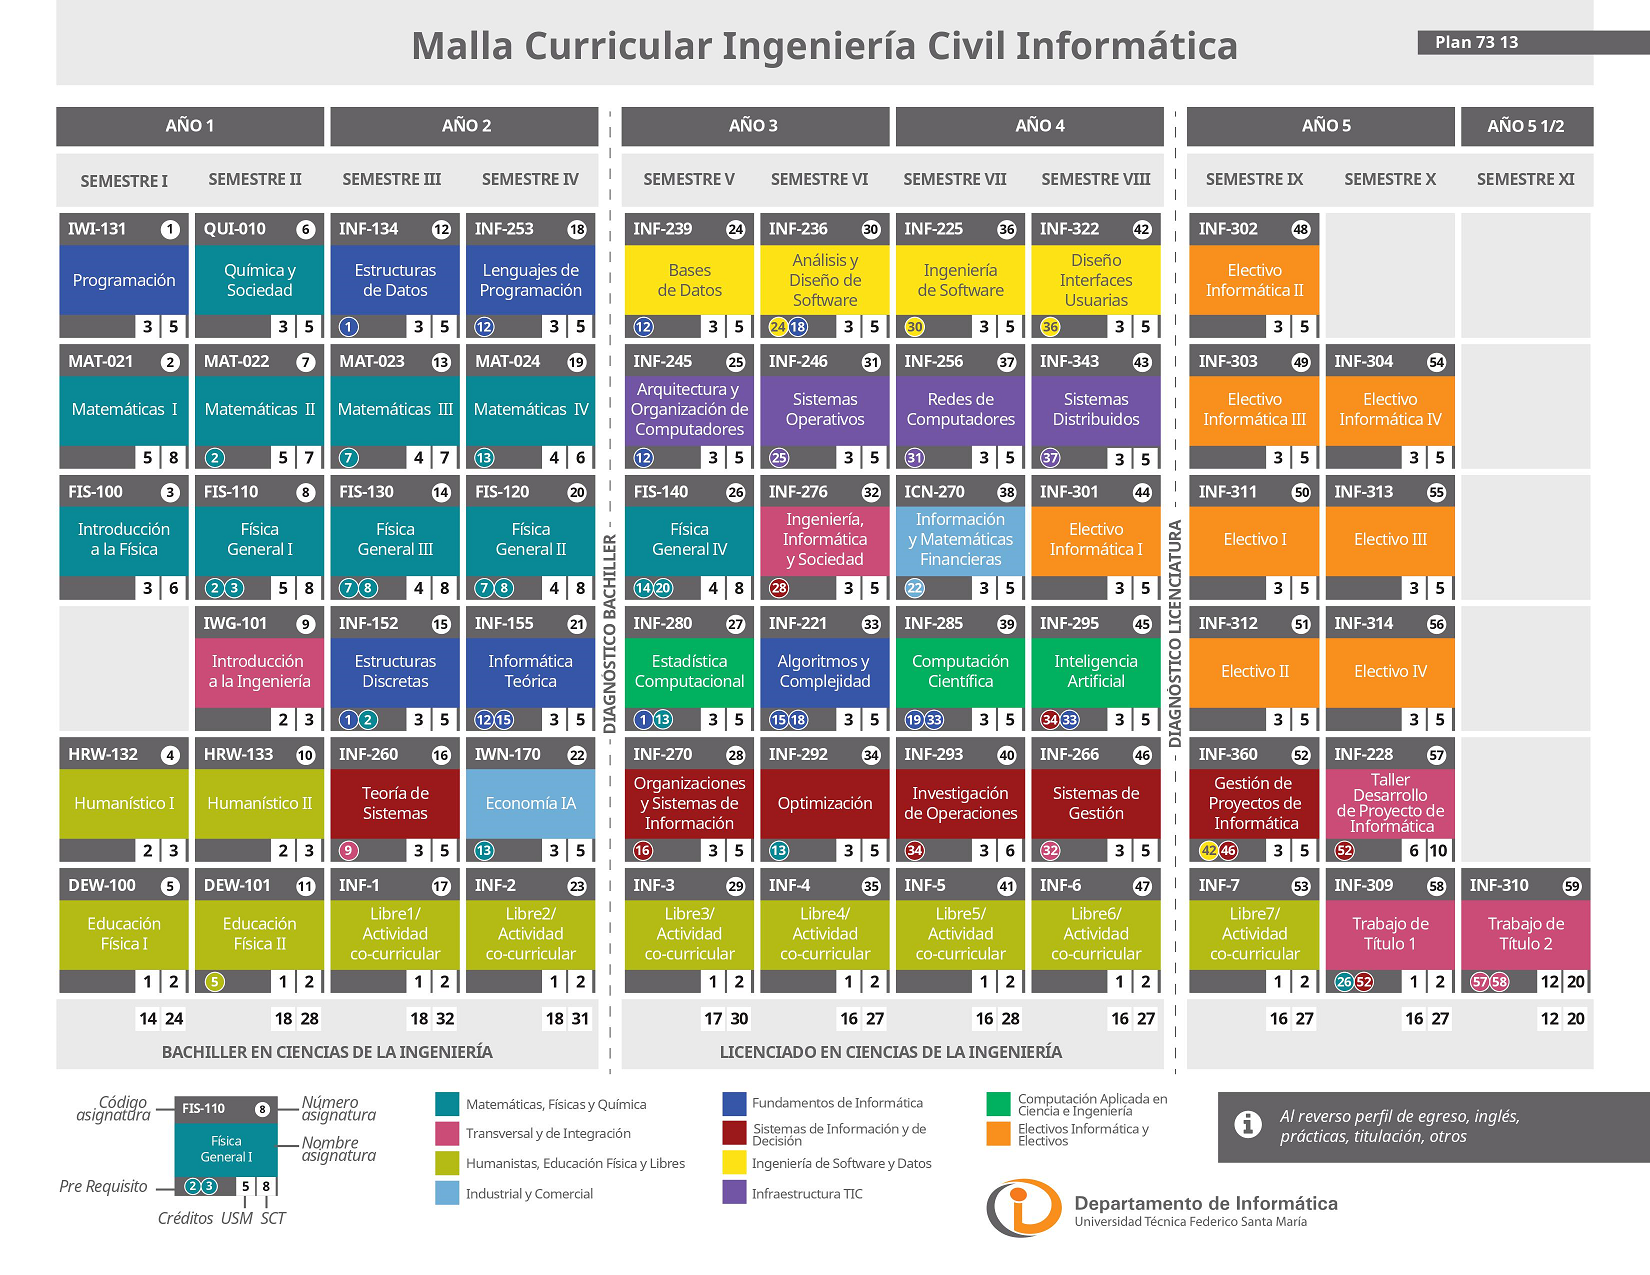
\includegraphics[width=0.8\textwidth]{malla_ingenieria_informatica}
% \caption{\label{fig:malla} Malla Curricular Ingeniería Civil Informática.} Fuente: Departamento de Informática.
% \end{figure}



% \begin{algorithm}
% \caption{Algoritmo de propuesta Donoso}\label{alg:propuesta_donoso} 
% \SetKwInOut{KwIn}{Input}
% \SetKwInOut{KwOut}{Output}
% % functions
% \SetKwFunction{generateMesh}{GENERATE\_MESH}
% \SetKwFunction{generateBalancedOctree}{GENERATE\_BALANCED\_OCTREE}
% \SetKwFunction{applyTransitionPatterns}{APPLY\_TRANSITION\_PATTERNS}
% \SetKwFunction{applySurfacePatterns}{APPLY\_SURFACE\_PATTERNS}
% \SetKwFunction{refineElement}{REFINE\_ELEMENT}
% \SetKwFunction{add}{ADD}
% \SetKwFunction{getBoundaryNodes}{GET\_BOUNDARY\_NODES}
% \SetKwFunction{getLabeledNodes}{GET\_LABELED\_NODES}
% % procedure
% \SetKwProg{myproc}{Procedure}{:}{}
% \KwIn{Refinement level constraints $RLC$, triangular surface mesh \Omega, quality threshold $T$, maximum number of iterations $I$.}
% \KwOut{if successful, volumetric mesh of \Omega that meet the $RLC$ with quality greather than $T$.}
% \myproc{\generateMesh{key, value}}
% {
%     $imesh$ \gets \generateBalancedOctree{RLC,\Omega}\;
%     $imesh$ \gets \applyTransitionPatterns{imesh}\;
%     $l$ \gets $empty set$ \;
%     \For{$1$ \textbf{to} $I$} {
%         $mesh$ \gets $imesh$ \;
%         $bnodes$ \gets \getBoundaryNodes{mesh, \Omega}\;
%         \For{ \textbf{each} $node$ \textbf{in} $bnodes$} {
%             \If{$node \in l$ \textbf{or} ($node$ is \textbf{inside} of \Omega \textbf{and} $node$ is \textbf{close} to \Omega)} {
%                 $node$.\refineElement{\Omega}\;
%             }
%         }
%         $mesh$ \gets \applySurfacePatterns{mesh}\;
%         $bnodes$ \gets \getBoundaryNodes{mesh, \Omega}\;
%         \For{\textbf{each} $node$ \textbf{in} $bnodes$} {
%             \If{$node$ is \textbf{outside} of \Omega} {
%                 $node$.\refineElement{\Omega}\;
%             }
%         }
%         $ln$ \gets \getLabeledNodes{mesh, $T$}\;
%         \If{$ln$ \textbf{is} empty}{
%             \KwRet mesh \;
%         }
%         \For{\textbf{each} $node$ in $ln$}{
%             $l$.\add(node)
%         }
%     }
%     \KwRet mesh\;    
% }
% \end{algorithm}


% \begin{algorithm}
% \caption{Algoritmo de propuesta Donoso}\label{alg:propuesta_donoso}
% \DontPrintSemicolon
% \SetKwInOut{KwIn}{Input}
% \SetKwInOut{KwOut}{Output}
% % functions
% \SetKwFunction{generateMesh}{GENERATE\_MESH}
% \SetKwFunction{refineOctant}{REFINE\_OCTANT}
% \SetKwFunction{generateBalancedOctree}{GENERATE\_BALANCED\_OCTREE}
% \SetKwFunction{applyTransitionPatterns}{APPLY\_TRANSITION\_PATTERNS}
% \SetKwFunction{applySurfacePatterns}{APPLY\_SURFACE\_PATTERNS}
% \SetKwFunction{refineOctant}{REFINE\_OCTANT}
% \SetKwFunction{add}{ADD}
% \SetKwFunction{getBoundaryNodes}{GET\_BOUNDARY\_NODES}
% \SetKwFunction{getLabeledOctants}{GET\_LABELED\_OCTANTS}
% \SetKwFunction{getRefinementLevel}{getRefinementLevel}
% % procedure
% \SetKwProg{myproc}{Procedure}{:}{}
% \KwIn{Restricciones de nivel de refinamiento $RLC$, malla de superficie triangular \Omega, umbral de calidad $T$, número máximo de iteraciones $I$.}
% \KwOut{Malla volumétrica de \Omega que cumpla con el $RLC$ con calidad superior a $T$.}
% \myproc{\generateMesh{key, value}}
% {
%     $imesh$ \gets \generateBalancedOctree{RLC,\Omega}\;
%     $imesh$ \gets \applyTransitionPatterns{imesh}\;
%     $l$ \gets empty set \tcp*{vector con octantes asociados a nodos de mala calidad.}
%     \For{$1$ \textbf{to} $I$} {
%         $mesh$ \gets $imesh$ \;
%         \tcc{Refinar octante asociado a nodo de mala calidad.}
%         \For{\textbf{each} $octant$ in $l$}{
%             $octant$.\refineOctant{\Omega}\;
%         }
%         \tcc{Obtener octantes con nodos de mala calidad.}
%         $lo$ \gets \getLabeledOctants{mesh, $T$}\;
%         \If{$lo$ \textbf{is} empty}{
%             \KwRet $mesh$ \;
%         }
%         \For{\textbf{each} $octant$ in $lo$}{
%             $l$.\add(octant)
%         }
%     }
%     \KwRet mesh\;    
% }
% \myproc{\refineOctant{\Omega}}
% {
%     $octant$ \gets this.octant \;
%     rl\_current \gets $octant$.\getRefinementLevel{} \;
    
% }
% \end{algorithm}


% \begin{algorithm}
% \SetKwInOut{KwIn}{Input}
% \SetKwInOut{KwOut}{Output}
% % functions
% \SetKwFunction{generateMesh}{GENERATE\_MESH}
% \SetKwFunction{generateBalancedOctree}{GENERATE\_BALANCED\_OCTREE}
% \SetKwFunction{applyTransitionPatterns}{APPLY\_TRANSITION\_PATTERNS}
% \SetKwFunction{applySurfacePatterns}{APPLY\_SURFACE\_PATTERNS}
% \SetKwFunction{projectOnto}{PROJECT\_ONTO}
% \SetKwFunction{add}{ADD}
% \SetKwFunction{getBoundaryNodes}{GET\_BOUNDARY\_NODES}
% % procedure
% \SetKwProg{myproc}{Procedure}{:}{}
% \KwIn{Refinement level constraints $RLC$, triangular surface mesh \Omega, quality threshold $T$, maximum number of iterations $I$.}
% \KwOut{if successful, volumetric mesh of \Omega that meet the $RLC$ with quality greather than $T$.}
% \myproc{\generateMesh{key, value}}
% {
%     $imesh$ \gets \generateBalancedOctree{RLC,\Omega}\;
%     $imesh$ \gets \applyTransitionPatterns{imesh}\;
%     $l$ \gets empty set \;
%     \For{$1$ \textbf{to} $I$} {
%         $mesh$ \gets $imesh$ \;
%         $bnodes$ \gets \getBoundaryNodes{mesh, \Omega}\;
%         \For{ \textbf{each} $node$ \textbf{in} $bnodes$} {
%             \If{$node \in l$ \textbf{or} ($node$ is \textbf{inside} of \Omega\, \& $node$ is \textbf{close} to \Omega)} {
%                 $node$.\projectOnto{\Omega} \;
%             }
%         }
%         $mesh$ \gets \applySurfacePatterns{mesh}\;
%         $bnodes$ \gets \getBoundaryNodes{mesh, \Omega}\;
%         \For{\textbf{each} $node$ \textbf{in} $bnodes$} {
%             \If{$node$ is \textbf{outside} of \Omega} {
%                 $node$.\projectOnto{\Omega} \;
%             }
%         }
%         \If{$ln$ \textbf{is} empty}{
%             \KwRet mesh \;
%         }
%         \For{\textbf{each} $node$ in $ln$}{
%             $l$.\add(node)
%         }
%     }
    
%     \KwRet null\;    
% }
% \caption{Algoritmo de propuesta Daines \\ Fuente: \cite{daines2018repairing}}
% \label{alg:propuesta_daines} 
% \end{algorithm}





% \begin{algorithm}
% \SetKwInOut{KwIn}{Input}
% \SetKwInOut{KwOut}{Output}
% % functions
% \SetKwFunction{main}{MAIN}
% \SetKwFunction{getInput}{GET\_INPUT}
% \SetKwFunction{generateMesh}{GENERATE\_MESH}
% \SetKwFunction{exportMesh}{EXPORT\_MESH}
% \SetKwFunction{saveData}{SAVE\_DATA}
% \SetKwFunction{generateBalancedOctree}{GENERATE\_BALANCED\_OCTREE}
% \SetKwFunction{applyTransitionPatterns}{APPLY\_TRANSITION\_PATTERNS}
% \SetKwFunction{applySurfacePatterns}{APPLY\_SURFACE\_PATTERNS}
% \SetKwFunction{projectOnto}{PROJECT\_ONTO}
% \SetKwFunction{add}{ADD}
% \SetKwFunction{getBoundaryNodes}{GET\_BOUNDARY\_NODES}
% % procedure
% \SetKwProg{myproc}{Procedure}{:}{}
% \KwIn{Refinement level constraints $RLC$, triangular surface mesh \Omega.}
% \KwOut{Volumetric mesh of \Omega that meets $RLC$.}
% \myproc{\main{argc}}
% {
%     $inputs$ \gets \getInput{argc}\;
%     $mesh$  \gets \generateMesh{inputs}\;
%     \exportMesh{mesh}\;
% }
% \caption{Algoritmo de generación de mallas Octree con elementos mixtos y varios niveles de refinamiento.\\ Fuente: \cite{daines2018repairing}}
% \label{alg:propuesta_daines} 
% \end{algorithm}